\documentclass[12pt]{article}
\usepackage[a4paper]{geometry}
\usepackage[utf8]{inputenc}
\usepackage{fancyhdr}
\usepackage{lastpage}
\usepackage{graphicx, wrapfig, subcaption, setspace, booktabs}
\usepackage{graphicx}
\usepackage[T1]{fontenc}
\usepackage[font=small, labelfont=bf]{caption}
\usepackage[protrusion=true, expansion=true]{microtype}
\usepackage[english]{babel}
\usepackage{sectsty}
\usepackage{url, lipsum}
\usepackage[T1]{fontenc}
\usepackage{icomma}
\usepackage{siunitx}
\usepackage{ragged2e}
\usepackage{amsmath}
\usepackage{comment}
\usepackage{enumerate}
\usepackage{anysize}


\newcommand{\HRule}[1]{\rule{\linewidth}{#1}}
\onehalfspacing
\setcounter{tocdepth}{5}
\setcounter{secnumdepth}{5}

\begin{document}

\begin{titlepage}

\title{ \normalsize 
        \begin{center}
        
\includegraphics[height=6cm]{logo.png}
        \end{center}
        \LARGE \textsc{\textbf{Universidad De Sonora}} \\ \bigskip
		\Large División de Ciencias Exactas y Naturales \\
        Licenciatura en Física \\ \bigskip
        \bigskip
        Física Computacional I
		\\ [0.1cm]  
		\HRule{2pt} \\
		\Large \textbf{{Actividad 6}} \\
        \textit{\textbf{"Sistema de resortes acoplados"}}
		\HRule{2pt} \\
		\normalsize \vspace*{0.001\baselineskip}}
        
\date{\bigskip \Large Hermosillo, Sonora  \hspace*{\fill}  19 de Marzo de 2018}

        
\author{
		\Large\textbf{ Michelle Contreras Cossio} \\ \bigskip
        \\ \bigskip
       \Large Profr. Carlos Lizárraga Celaya}
       \end{titlepage}
       \maketitle
       

\newpage
\pagestyle{plain}

\section{Introducción}
El presente reporte muestra el procedimiento y resultados obtenidos al realizar la actividad \#6 de la clase Física Computacional I. El objetivo de la práctica es continuar con el uso de phyton, enfocandonos en la simulación de cierto fenómeno físico, para poder comparar soluciones numéricas con analíticas. \\

Durante esta semana se trabajó con jupyter lab, otra forma de trabajar con phyton, donde tenemos un mayor acercamiento a los archivos con los que trabajamos, una interfaz un poco diferente y con otras funcionalidades. \\

Además, se utilizó el artículo de "Coupled spring equations" para simular, con ayuda de phyton, sistemas de resortes acoplados, para obtener gráficas identicas a las del artículo. 

\section{Síntesis de "Coupled spring equations"}

En esta sección mostramos una síntesis de artículo "Coupled spring equations" por Temple H. Fay y Sarah Duncan Graham. Además se añade el código utilizado para resolver estos mismos problemas, haciendo uso de jupyter lab.

\subsection{Introducción}
En este artículo, se trata el problema de dos resortes y dos masas, conectados en serie y suspendidos desde el techo. Para resolver este fenómeno, se hace uso de la Ley de Hooke, para la fuerza restauradora del resorte, lo que resulta en la solución de ecuaciones diferenciales lineales de segundo orden, sin embargo, se pueden llegar a convertir en ecuaciones diferenciales lineales de hasta cuarto orden.\\ 

A partir de estas ecuaciones se pueden tener muchas interpretaciones físicas, sobre la fase o desfase, además que se pueden agregar términos como uno no lineal, que pretende mostrar algo físicamente más viable. \\

En resumen, podemos modificar fácilmente variables como la periodicidad, fase, amplitud, entre otras, modificando simplemente las ecuaciones.

\subsection{El modelo de resortes acoplados}

Este modelo consiste en dos resortes y dos masas, valores de k y m diferentes, colgados al techo y movidos desde su posición de equilibrio en x. 

\subsubsection{Asumiendo la Ley de Hooke}

Tomando como cierta la Ley de Hooke, cada resorte estirados tendrá una fuerza restauradora de -kx, donde k es la constante del resorte y x es lo que se estiró. 

\begin{center}
        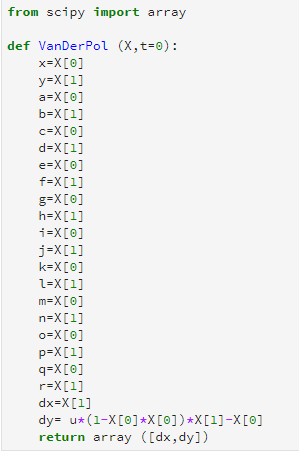
\includegraphics[height=6cm]{1.png}
\end{center}

La masa superior siente dos fuerzas, puesto que se encuentra entre dos resortes, la propia al resorte superior y una fuerza hacia arriba por la resistencia del segundo resorte para ser estirado. Mientras que la masa inferior únicamente siente la fuerza del resorte al cual se encuentra conectado. De esta manera, gracias a la Ley de Newton, podemos representar lo dicho en dos ecuaciones:

\begin{equation}
m_1 \ddot x_1 = -k_1x_1 - k_2(x_1-x_2)
\end{equation}

\begin{equation}
m_2 \ddot x_2 = -k_2(x_2-x_1)
\end{equation}

Si se buscara encontrar una ecuación para $x_1$, de modo que no se involucrara a $x_2$, y viceversa se obtienen dos ecuaciones lineales de cuarto grado, a las cuales se llega, despejando una variable de la primera ecuación y sustituyendo en la segunda:\\

\centerline{$m_1m_2x_1^{(4)} + (m_2k_1 + k_2(m_1+m_2)) \ddot x_1 + k_1k_2x_1=0$}
\centerline{$m_1m_2x_2^{(4)} + (m_2k_1 + k_2(m_1+m_2)) \ddot x_2 + k_1k_2x_2=0$}
.\\
Ecuaciones con las cuales, solamente se hace uso de los desplazamientos y velocidades iniciales. Así pues, una alternativa que se tiene es convertir el sistema de dos ecuaciones de segundo orden a uno de 4 ecuaciones de cuarto orden. Sin embargo, en los ejemplos se trabajara con el primer sistema. 

\subsubsection{Ejemplos} 
Los siguientes ejemplos muestran el uso de dos masas $m_1$ = $m_2$ = 1. Sin fricción ni fuerza externa, haciendo uso de las ecuaciones (1) y (2).

\begin{itemize}
\item \textbf{Ejemplo 2.1}

Describir el movimiento de los resortes con $k_1$=6, $k_2$=4 y condiciones iniciales $(x_1(0), \dot x_1(0), x_2(0), \dot x_2(0))$ = (1, 0, 2, 0).\\

Resolviendo las ecuaciones, se llegó a que la solución analítica para este problema es: \\

\centerline{$x_1(t) = cos\sqrt (2t)$}
\centerline{$x_2(t) = 2cos\sqrt (2t)$}

Este movimiento es sincronizado y se encuentra en fase, las masas tienen el mismo período, esto se puede ver en la gráficas creadas, mostradas a continuación. 

\begin{itemize}
\item \textbf{Solución numérica con Phyton:}

NOTA: El código mostrado a continuación, así como el que produce las gráficas, se utilizó de manera idéntica para los ejemplos 2.1, 2.2 y 2.3, cambiando únicamente las condiciones iniciales (celda 2):

Lo que hace este código es crear vectores que obtengan los valores para las velocidades, posiciones, masas, constantes de los resortes, etc.

\begin{center}
        
\includegraphics[height=6cm]{2.png}
\end{center}

Posteriormente se tiene una sección que permite dar los valores iniciales de masas, constantes, etc. Se crea un archivo de datos, con tiempos que van cambiando según se asigne, que contiene tiempos, velocidad y posición a cierto tiempo y el error (en este caso y en el ejemplo 2.2). 

\begin{center}
        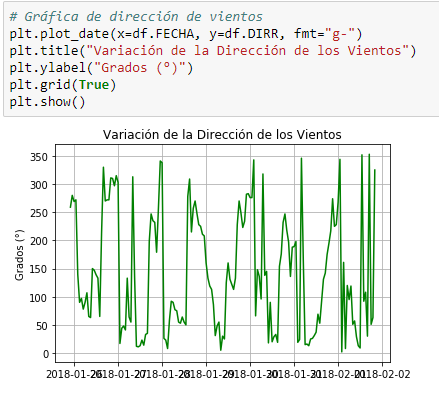
\includegraphics[height=14cm]{3.png}
\end{center}


A partir de ese archivo se crearon las gráficas, utilizando algunas de las variables que contenga. 

\clearpage
Así se produjo el movimiento de $x_1$ y de $x_2$ a través del tiempo:

\begin{center}
        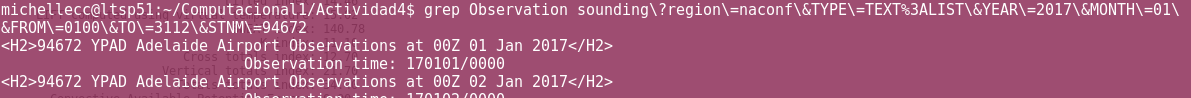
\includegraphics[height=7cm]{4.png}
\end{center}

Dando como resultado:

\begin{center}
        \includegraphics[height=6cm]{ej2_1_1.png}
\end{center}


Así se produjo la fase de $x_1$ y de $x_2$ (v vs x):

\begin{center}
        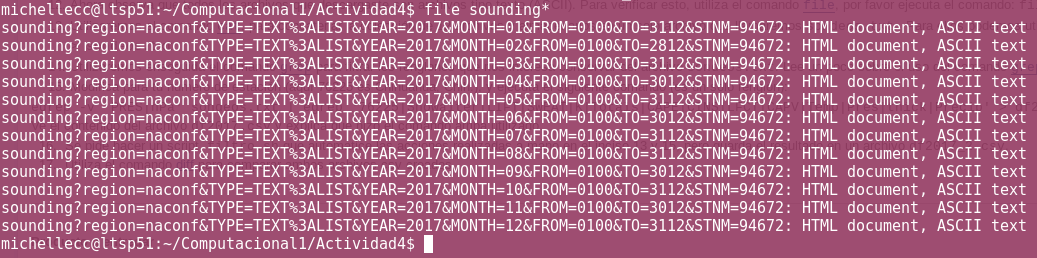
\includegraphics[height=7cm]{5.png}
\end{center}

Dando como resultado:

\begin{center}
        \includegraphics[height=6cm]{ej2_1_2.png}
\end{center}

Así se produjo $x_1$ y vs $x_2$:

\begin{center}
        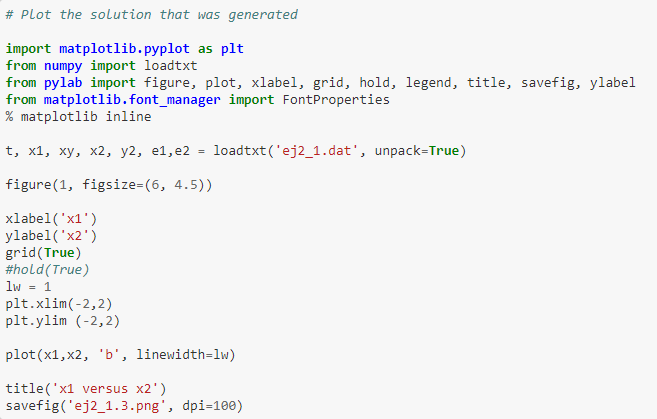
\includegraphics[height=7cm]{6.png}
\end{center}

Dando como resultado:


\begin{center}
        \includegraphics[height=6cm]{ej2_1_3.png}
\end{center}

\item \textbf{Calculo del error}

Para calcular el error, primeramente, se agregaron al archivo creado dos columnas,una para el error con respecto a $x_1$ y otra para el error con respecto a $x_2$, esos errores se calcularon restando a la x correspondiente a cierto tiempo (valor numérico), la función solución evaluada en el mismo tiempo (valor analítico),y dividiendolo entre este valor analítico. 


\begin{center}
        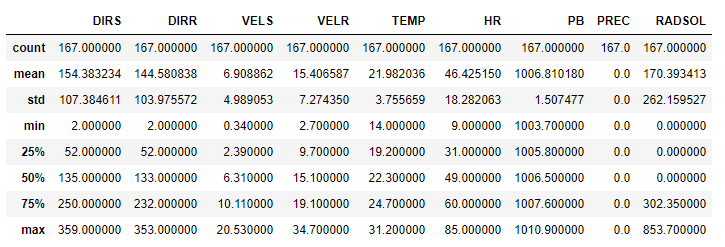
\includegraphics[height=2cm]{7.png}
\end{center}

\begin{center}
        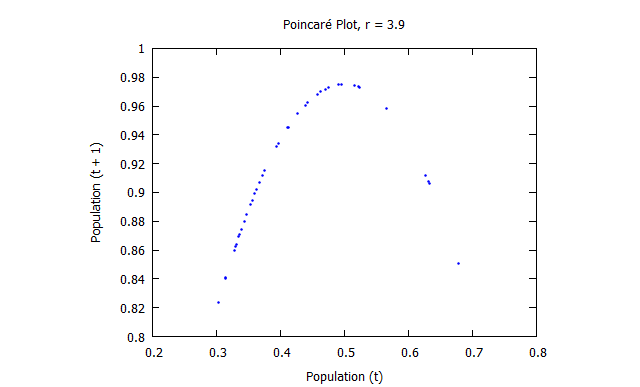
\includegraphics[height=7cm]{8.png}
\end{center}

Posteriormente, se graficaron ambos errores con respecto del tiempo:

\begin{center}
        \includegraphics[height=6cm]{error2_1.png}
\end{center}

\end{itemize}

\item \textbf{Ejemplo 2.2}

Describir el movimiento de los resortes con $k_1$=6, $k_2$=4 y condiciones iniciales $(x_1(0), \dot x_1(0), x_2(0), \dot x_2(0))$ = (-2, 0, 1, 0).\\

Resolviendo las ecuaciones, se llegó a que la solución analítica para este problema es: \\

\centerline{$x_1(t) = -2cos (2\sqrt (3t))$}
\centerline{$x_2(t) = cos (2\sqrt (3t))$}

Lo que representa que cuando una masa se mueve para arriba, la otra se mueve para abajo, pero tienen el mismo período, con un desfase de 180$^\circ$

\begin{itemize}
\item \textbf{Solución numérica con Phyton}

Se utilizó el mismo código utilizado en el ejemplo anterior, pero únicamente se produjeron las gráficas de el movimiento de $x_1$ y de $x_2$ a través del tiempo:


\begin{center}
        \includegraphics[height=6cm]{ej2_2_1.png}
\end{center}

y de $x_1$ y vs $x_2$:


\begin{center}
        \includegraphics[height=6cm]{ej2_2_2.png}
\end{center}

\item \textbf{Cálculo del error}
\end{itemize}

El error se produjo de la misma manera que en el ejemplo anterior, utilizando ahora las nuevas soluciones analíticas, la gráfica obtenida fue la siguiente:


\begin{center}
        \includegraphics[height=6cm]{error2_2.png}
\end{center}

\item \textbf{Ejemplo 2.3}

Describir el movimiento de los resortes con $k_1$=0.4, $k_2$=1.808 y condiciones iniciales $(x_1(0), \dot x_1(0), x_2(0), \dot x_2(0))$ = (1/2, 0, -1/2, 7/10).\\

Cambiando estos valores iniciales, únicamente va a cambiar el período y la frecuencia, así como la amplitud y fase en la soluciones. Con los programas que creamos podemos verificar eso al variar los valores de k. 

\begin{itemize}
\item \textbf{Solución numérica con Phyton}

Se realizaron básicamente las mismas gráficas que se crearon en los ejemplos anteriores.

Primeramente se crearon las gráficas de fase, una para $x_1$ y otra para $x_2$, esta vez se encuentra cada uno en una gráfica.

\begin{figure}[h!]
\begin{subfigure}{.55\textwidth}
\centering
\includegraphics[width=1\linewidth]{ej2_3_1.png}
\end{subfigure}
\begin{subfigure}{.55\textwidth}
\centering
\includegraphics[width=1\linewidth]{ej2_3_2.png}
\end{subfigure}
\end{figure}

\clearpage
Posteriormente el plot de $x_1$ y $x_2$, por separado con respecto al tiempo. 

\begin{figure}[h!]
\begin{subfigure}{.55\textwidth}
\centering
\includegraphics[width=1\linewidth]{ej2_3_3.png}
\end{subfigure}
\begin{subfigure}{.55\textwidth}
\centering
\includegraphics[width=1\linewidth]{ej2_3_4.png}
\end{subfigure}
\end{figure}

El movimiento de $x_1$ y $x_2$ con respecto al tiempo, en una sola.

\begin{center}
        \includegraphics[height=6cm]{ej2_3_5.png}
\end{center}

Plot de $x_1$ vs $x_2$.

\begin{center}
        \includegraphics[height=6cm]{ej2_3_6.png}
\end{center}

\end{itemize}


\end{itemize}

\subsubsection{Amortiguamiento}
El tipo de amortiguamiento (o fricción para el caso en el que las masas se encuentran sobre alguna superficie) con el que estaremos trabajando es el viscoso, que depende únicamente de la velocidad. En este caso, que tenemos dos resortes, el amortiguamiento de la primera masa depende únicamente de su velocidad y no de la velocidad de la otra masa y viceversa. \\

Así, añadiendo el término de amortiguamiento, las ecuaciones quedan:

\begin{equation}
m_1 \ddot x_1 = -\delta _1 \dot{x_1} -k_1x_1 - k_2(x_1-x_2)
\end{equation}
\begin{equation}
m_2 \ddot x_2 = -\delta _2 \dot{x_2} -k_2(x_2-x_1)
\end{equation}

De igual manera que en el movimiento de dos resortes acoplados simples, se puede modificar el sistema que tenemos de dos ecuaciones de segundo grado a un sistema de cuatro ecuaciones de cuarto grado, sin embargo, trabajaremos con el que ya tenemos. 

\begin{itemize}
\item \textbf{Ejemplo 2.4}

Describir el movimiento de los resortes con $m_1 = m_2 = 1$, $k_1$=0.4, $k_2$=1.808, constantes de amortiguamiento $\delta _1$= 0.1, $\delta _2$= 0.2 y condiciones iniciales $(x_1(0), \dot x_1(0), x_2(0), \dot x_2(0))$ = (1, 1/2, 2, 1/2).

El amortiguamiento va a causar que poco a poco la amplitud del movimiento disminuya. 

\begin{itemize}
\item \textbf{Solución numérica con Phyton}

El código utilizado sigue siendo el mismo, únicamente se tiene que en este caso si existirán coeficientes de fricción/ amortiguamiento.
Se crearon las mismas gráficas del ejemplo anterior.

Gráficas de fase, una para $x_1$ y otra para $x_2$.

\begin{figure}[h!]
\begin{subfigure}{.45\textwidth}
\centering
\includegraphics[width=1\linewidth]{ej2_4_1.png}
\end{subfigure}
\begin{subfigure}{.45\textwidth}
\centering
\includegraphics[width=1\linewidth]{ej2_4_1.png}
\end{subfigure}
\end{figure}

Plot de $x_1$ y $x_2$
\begin{figure}[h!]
\begin{subfigure}{.55\textwidth}
\centering
\includegraphics[width=1\linewidth]{ej2_4_3.png}
\end{subfigure}
\begin{subfigure}{.55\textwidth}
\centering
\includegraphics[width=1\linewidth]{ej2_4_4.png}
\end{subfigure}
\end{figure}

El movimiento de $x_1$ y $x_2$ con respecto al tiempo

\begin{center}
        \includegraphics[height=6cm]{ej2_4_5.png}
\end{center}

Plot de $x_1$ vs $x_2$.

\begin{center}
        \includegraphics[height=6cm]{ej2_4_6.png}
\end{center}

\end{itemize}

\end{itemize}

\section{Conclusiones}

Primeramente, me gustaría hablar del entorno Jupyter Lab, me pareció muy bueno, ya que cuenta con todo lo que se necesita en una sola ventana, cuenta con un navegador de archivos que es realmente útil. Me gustó más que el anterior. \\

Por otro lado, fue interesante trabajar por primera vez con simulación numérica, cosa que no se había trabajado como tal, pudiendo relacionar cosas que ya hemos aprendido, tanto en esta como en otras materias. 

\section{Bibliografía}

\begin{itemize}
\item Ley de elasticidad de Hooke (2018). Consultado: 25 de Marzo del 2018, de Wikipedia. Sitio web: https://es.wikipedia.org/wiki/Ley\_de\_elasticidad\_de\_Hooke
\item Couple spring equations (2003).Temple H. Fay, Sarah Duncan Graham. Consultado: 27 de Marzo del 2018, de Oregon State University. Sitio web:  http://math.oregonstate.edu/\\
\~gibsonn/Teaching/MTH323-010S15/Supplements/coupled\_spring.pdf
\end{itemize}

\section{Apéndice}

\begin{enumerate}
\item ¿En general te pareció interesante esta actividad de modelación matemática? ¿Qué te gustó mas? ¿Qué no te gustó?

Si me pareció interesante, me gustó poder resolver problemas de una manera numérica, como en la clase de análisis numérico, ya que en ocasiones dejamos de lado estas soluciones, que en realidad son muy útiles.

\item La cantidad de material te pareció ¿bien?, ¿suficiente?, ¿demasiado?

Me pareció suficiente, aunque tarde bastante en realizar la actividad.

\item ¿Cuál es tu primera impresión de Jupyter Lab? 

Bastante útil, manejable y todo se encuentra en una sola ventana, cosa que me agrada mucho, tener todo a la mano.

\item Respecto al uso de funciones de SciPy, ¿ya habías visto integración numérica en tus cursos anteriores? ¿Cuál es tu experiencia?.

Si, en cálculo y análisis numérico. Este método te lo realiza todo en automático, ya que antes lo teníamos que realizar todo, sin una función, ya fuera a mano o computadora.

\item El tema de sistema de masas acopladas con resortes, ¿ya lo habías resuelto en tu curso de Mecánica 2?  

Si, pero creo que con amortiguamiento no.

\item ¿Qué le quitarías o agregarías a esta actividad para hacerla más interesante y divertida?

Me pareció justo el tema y el contenido que tiene. 

\end{enumerate}
\end{document}